%%%%%%%%%%%%%%%%%%%%%% Props %%%%%%%%%%%%%%%%%%%%%%
\documentclass{article}

\usepackage[french]{babel}
\usepackage[utf8]{inputenc}
\usepackage[T1]{fontenc}
\usepackage{graphicx}
\usepackage{fancyhdr}
\usepackage{eurosym}
\usepackage{color}
\usepackage{soul}
\usepackage{listings}
\usepackage{enumitem}
\usepackage{enumerate}

\pagestyle{fancy}
\lhead{Cahier des charges}
\chead{Deadly Science}
\rhead{Custos Carceris}

\definecolor{mygreen}{rgb}{0,0.6,0}
\definecolor{mygray}{rgb}{0.5,0.5,0.5}
\definecolor{mymauve}{rgb}{0.58,0,0.82}

\lstset{ 
  commentstyle=\color{mygreen},
  keywordstyle=\color{blue},       % keyword style
  numberstyle=\tiny\color{mygray}, % the style that is used for the line-numbers
  rulecolor=\color{black},         % if not set, the frame-color may be changed on line-breaks within not-black text (e.g. comments (green here))
  stringstyle=\color{mymauve},     % string literal style
  language=[Sharp]C,                 % the language of the code
  backgroundcolor=\color{white},   % choose the background color; you must add \usepackage{color} or \usepackage{xcolor}; should come as last argument
  basicstyle=\footnotesize,        % the size of the fonts that are used for the code
  breakatwhitespace=true,         % sets if automatic breaks should only happen at whitespace
  breaklines=true,
  extendedchars=true,              % lets you use non-ASCII characters; for 8-bits encodings only, does not work with UTF-8
  frame=single,	                   % adds a frame around the code
  tabsize=2,	                   % sets default tabsize to 2 spaces
  showstringspaces=false,
}

\begin{document}


%%%%%%%%%%%%%%%%%%%%%% Titre %%%%%%%%%%%%%%%%%%%%%%
\begin{titlepage}
	\centering
	{\scshape\LARGE Custos Carceris\par}
	\vspace{1cm}
	{\scshape\Large Première soutenance \par}
	\vspace{1.5cm}
	{\huge\bfseries Deadly Science\par}
	\vspace{2cm}
	
\includegraphics[width=0.5\textwidth]{logo.png}\par\vspace{1cm}
	{\Large\itshape Léandre Perrot\par}
	{\Large\itshape Yann Boudry\par}
	{\Large\itshape Steve Suissa\par}
	{\Large\itshape Célian Raimbault\par}
	\vfill
	Un projet EPITA
	\vfill
	{\large \today\par}
\end{titlepage}



\newpage
\tableofcontents


%%%%%%%%%%%%%%%%%%%%%% Intro %%%%%%%%%%%%%%%%%%%%%%

\section{Introduction}

\newpage
\section{Réalisations}

%%%%%%%%%%%%%%%%%%%%%% Yann %%%%%%%%%%%%%%%%%%%%%%

\subsection{Yann Boudry}

\subsubsection{Menu Principal}

Le menu est la première image qu'aperçoit le joueur du jeu. Il est important d'avoir un menu bien réalisé et qui donne envie de jouer à l'utilisateur.

\par\vspace{0.5cm}
\begin{figure}[!h]
    \centering
    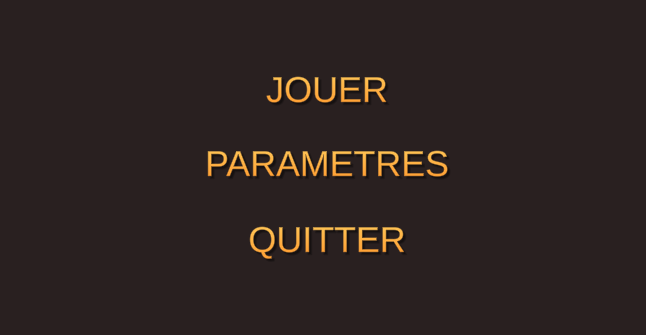
\includegraphics[width=0.5\textwidth]{MainMenu.png}
    \caption{Main Menu}
    \label{Main Menu}
\end{figure}{}

\paragraph{Menu}

J'ai choisi de faire un menu simple qui comporte les fonctionalité essentielles que l'on attend de cette partie du jeu. Il comporte donc trois boutons:

\begin{itemize}
    \item Jouer, qui comme il l'indique permet de lancer une partie.
    \item Paramètres, qui là encore ouvre une fenêtre de paramètres.
    \item Quitter, comme son nom l'indique, il arrête l'application.
\end{itemize}

\subsubsection{Jouer}

\paragraph{}
Ce premier bouton vous approche d'un pas de plus vers l'épreuve de survie où tous les coups sont permis: Deadly Science. Après vous être lancé dans l'aventure apparaît un deuxième menu qui regroupe les différents laboratoires abandonnés de Deadly Science. Vous pouvez rejoindre un groupe partant pour une destination connue, ou bien-sûr en chercher un nouveau et l'explorer avec votre équipe. Mais gare aux maladies qui peuvent être... Mortelles!
\paragraph{} Si l'aventure vous effraie trop, vous pouvez toujours revenir en arrière pour parfaire la maîtrise de votre personnage au sein des paramètres ou tout simplement quitter le jeu.

\subsubsection{Paramètres}
Cette partie concerne les paramètres du jeu, pour l'instant ne comprenant qu'un gestionnaire de touches pour les différents mouvements (avant, arrière, gauche, droite, sauter).

\paragraph{Principe}
Unity propose un gestionnaire de touches mais il faut pour cela avoir le projet et l'éxecuter dans Unity.
Il est impossible de changer les touches une fois que le jeu est lancé. J'ai donc cherché des manières de remédier à ce problème.

\paragraph{Implémentation}

\subparagraph{Rebind}
Rien de plus énervant que de lancer son jeu favori mais de devoir réassigner les touches de son clavier à chaque fois. Afin d'empêcher toute destruction inopinée de materiel informatique j'ai écrit un script pour cela: InputManager. Il rassemble les touches utilisées et enregistrées, une fonction retournant la/les touches enfoncées, une autre retournant la touche associée à l'action demandée pour l'affichage et le changement de touches.
\newline Pour gérer et enregistrer les touches, j'ai utilisé un dictionaire de string/Keycode auquel j'attribue des valeurs par défaut dès que le script est appelé:

\begin{itemize}
    \item Jump => Espace
    \item Forward => W
    \item Backward => S
    \item Left => A
    \item Right => D
\end{itemize}

J'ai opté pour l'utilisation des PlayerPrefs pour la sauvegarde des touches car c'est une classe très facile à manipuler. Elle ne permet de stocker que des string, float ou int mais la conversion est très simple puisqu'il est possible de convertir les Keycodes en un int unique à l'aide d'un simple cast.
\newline Le script va ensuite tester l'existence de PlayerPrefs sur l'ordinateur de l'utilisateur auquel cas les touches prendront ces valeurs.

\par\vspace{0.2cm}
\begin{lstlisting}
    for (int i = 0; i < buttonKeys.Count; i++)
        {
            if (PlayerPrefs.HasKey(keys[i]))
                buttonKeys[keys[i]] = 
                    (KeyCode) PlayerPrefs.GetInt(keys[i]);
        }
\end{lstlisting}

Finalement, on sauvegarde les touches. (Utile seulement lors d'un premier lancement du jeu)

\subparagraph{En jeu}
J'ai également du refaire une fonction qui teste quand les touches sont enfoncées. Pour éviter de devoir changer les touches dans tout le code à chaque modification, elle prend le nom de l'action en argument et retourne l'état de la touche correspondante grâce au dictionnaire.

\subparagraph{Affichage}
Le panneau de paramètres utilise un script KeybindDialog qui récupère les noms des touches à partir de l'InputManager. Il va ensuite instancier un préfab pour chaque touche, constitué du nom de l'action et d'un bouton avec la touche correspondante. Lorsque ce bouton est appuyé il va écouter tout le clavier et réassigner la première touche enfoncée à l'action demandée. Le changement est sauvegardé sur l'ordinateur avec les PlayerPrefs en simultané pour la prochaine utilisation.

\subsubsection{Pause}

\par\vspace{0.5cm}
\begin{figure}[!h]
    \centering
    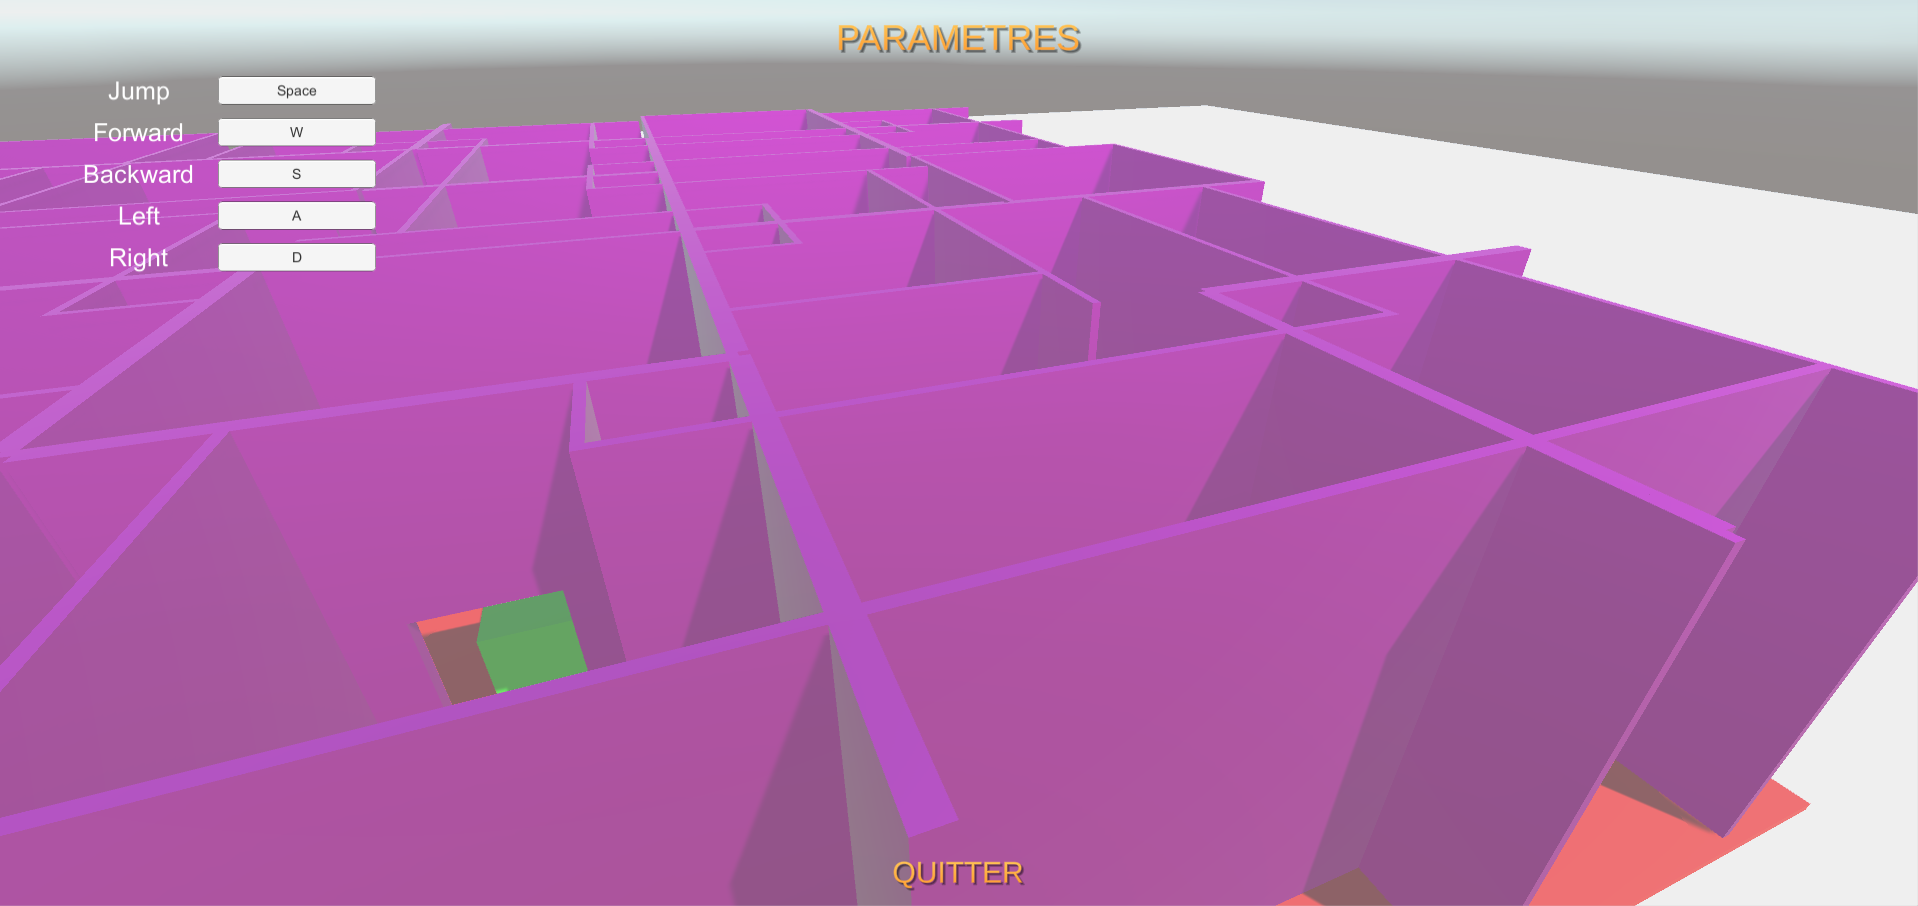
\includegraphics[width=1\textwidth]{Pause.PNG}
    \caption{"Pause"}
    \label{Pause}
\end{figure}{}

Un jeu n'existe pas sans son menu pause. Enfin... la pause dans un jeu en ligne est discutable.
On y retrouve les paramètres pour changer les touches enrichies d'un bouton quitter pour abandonner ses frères d'armes à leur sort et revenir au chaud du menu principal.

\subsubsection{Écran de fin}
%%%%%%%%%%%%%%%%%%%%%% Leandre %%%%%%%%%%%%%%%%%%%%%%
%%%%%%%%%%%%%%%%%%%%%% Celian %%%%%%%%%%%%%%%%%%%%%%

\newpage
\subsection{Célian Raimbault}

Dans ce projet, je suis chargé d'implémenter en priorité le comportement des joueurs, la musique et les effets. Pour cette soutenance je me suis concentré exclusivement sur le joueur car la musique et les effets serviront à rendre plus agréable le jeu une fois que nous aurons implémenter la base du jeu, c'est-à-dire prinicipalement le réseau avec le contrôle du joueur.

\subsubsection{Gameplay du joueur}

Le gameplay du joueur est un des points les plus important du jeu, de plus, il est important de commencer ce projet avec celui-ci. Cette partie se décompose en deux sous parties, la gestion de la physique ainsi que l'intéraction entre le joueur et l'environnement.

\paragraph{Gestion de la physique}

La physique du joueur est la première chose à implémenter car sans elle il n'y aurait pas de mouvements des joueurs et encore moins d'intéraction.
De plus, cette partie doit être réalisée avec minutie car elle peut radicalement changer le gameplay si elle est bien (ou mal) réalisée.

\subparagraph{Les physiques de Unity}

Unity dispose d'un moteur physique, c'est lui que nous utilisons car il est très complêt et adapté pour notre jeu. En effet, ce moteur physique nous permet d'appliquer des forces sur des objets, de tester si plusieurs objets sont en collision et même de définir des couches permettant de filtrer les collisions entre objets. Dans Unity, un objet peut avoir un corps s'il est dynamique (c'est à dire qu'il réagit à des forces extérieures) avec un ou plusieurs boîtes de collision.

\subparagraph{Principe}

En premier temps, j'ai pensé à définir le joueur avec un RigidBody et un boite de collision en forme de capsule, c'est à dire que le joueur est attiré vers le bas par la gravité et a une forme de capsule pour éviter de bouger quand il tourne et pour mieux pouvoir grimper sur des objets en sautant. Pour bouger le joueur, il suffit de tester à chaque mise à jour du jeu si une entrée clavier est appuyée et appliquer une force. Finalement, après avoir implémenté ce mécanisme je me suis rendu compte que Unity disposait également d'un composant nommé PlayerController et qu'il était peut être plus adapté au jeu. En effet, le PlayerController remplace le RigidBody du joueur, il permet d'entièrement contrôler le joueur, c'est à dire que c'est le rôle du développeur de gérer les physiques comme les forces appliquées sur le corps. Le PlayerController prends juste en charge les collisions entre les autres objets pour ne pas passer au travers. Il est préférable d'utiliser ce composant car nous pouvons par exemple enlever la gravité ou les forces de friction quand nous le voulons. Il est utilisé également pour éviter des bugs causés par le réseau, si deux joueurs sont au même endroit, il ne faut pas les éjecter.

\subparagraph{Implémentation}


J'ai ainsi déclaré un attribut \emph{velocity} au joueur qui est sa vitesse et ajoute une force de gravité à celui-ci. À chaque mise à jour du jeu, cette variable s'ajoute à la position du joueur, elle est juste multipliée par le temps qui s'est écoulé entre la dernière mise à jour pour que le mouvement soit fluide.

\begin{lstlisting}
Vector3 movements = x * transform.right + z * transform.forward;
\end{lstlisting}

Les mouvements se font presque de la même manière qu'avec un RigidBody, quand il y a une entrée active, ou ajoute à \emph{velocity} une force proportionnelle au temps de pression orientée vers la direction voulue. Il y a également une variable \emph{maxSpeed} qui est la limite de vitesse, si le joueur dépasse cette limite il ne peut que freiner son mouvement, c'est à dire que le produit scalaire entre \emph{velocity} et \emph{mouvement} doit être négatif pour mettre à jour la vitesse.

\emph{(Voir annexe [\ref{Mouvements}])}

Pour pouvoir sauter, il a fallu tester si le joueur touchait sol. Pour cela, j'ai ajouté un objet vide qui décrit la position de détection du sol comme ça le joueur teste si le sol est présent dans une petite sphère autours de ce point.

\begin{lstlisting}
bool grounded = velocity.y <= .1f &&
	Physics.CheckSphere(groundSensor.position, controller.radius, groundMask);
\end{lstlisting}

Il faut ajouter une force de frottements (provenant de l'air ou du sol) pour que le jeu soit jouable, sinon notre joueur ne s'arrêtera pas. Bien sûr, cette force est appliquée seulement si le joueur n'avance pas.

\emph{(Voir annexe [\ref{Friction}])}

Il est évident que le joueur n'est pas censé pouvoir grimper sur un autre joueur ou même sauter depuis un objet qui n'entre pas en collision avec lui. C'est pour cela que j'ai mis en place le système de couches physiques. Il y a, en plus de celles fournies par défaut par Unity, les couches :
- Player : Seulement pour les joueurs.
- Walls : Pour la détection du sol ou des murs.
- PowerUps : Ils ne touchent que les joueurs en tant que \emph{trigger}, c'est à dire que le joueur passe néanmoins au travers.

\paragraph{Intéraction joueur / environnement}

L'environnement comprends les sérums mais aussi les autres joueurs, le comportement des sérums face au joueur est plutôt simple alors commençons par celui-ci.

\subparagraph{Sérums}

Nous avons pensé qu'il serait envisageable d'ajouter des power ups à notre jeu une fois que celui ci sera plus complet, un sérum peut être considéré comme un power up car c'est un objet qui peut se faire collecter par un joueur. Pour éviter de changer beaucoup de script si nous ajoutons des power ups j'ai pensé à utilisé de la programmation orientée objet en créant une classe PowerUp qui est abstraite, elle possède une méthode \emph{OnCollect} qui est appelée lors d'une collision avec un joueur, elle prends en paramètre le joueur et retourne si le power up doit être détruit. Il ne doit pas toujours se détruire car un joueur ayant déjà collecté un sérum ne peut pas en prendre en autre. Le sérum utilise alors cette fonction dans sa propre classe.

\begin{lstlisting}
protected abstract bool PowerUp.OnCollect(GameObject player);
\end{lstlisting}


\paragraph{Joueur et réseau}

Le joueur est un des éléments les plus utilisés en réseau, sa position doit être synchronisée mais pas seulement, il faut prévenir chaque joueur quand un joueur change de status ou même se fait toucher par un autre joueur. Unity utilise des composants attribués aux objets en jeu, nous pouvons en mettre plusieurs pour un seul objet et c'est cela que nous allons faire pour le joueur. Le but est d'enlever les composants inutiles, par exemple, un joueur controllera un seul joueur en jeu donc le module gérant les mouvements du joueur sera retiré pour les joueurs non controllés. Ceci permet également de préparer le joueur dans une unique prefab en ajoutant tous les modules avec les bonnes propriétés.
Cette partie est particulièrement compliquée à imaginer quand on ne s'y connait pas bien en réseau, c'est pour cela qu'il est possible que certaines classes soit modifiées lors d'une future soutenance.

\subparagraph{Classes du joueurs}

\begin{itemize}
\item PlayerNetwork : Permet de gérer les événements liés au réseau et également met en place ou retire tous les autres classes du joueur. Ce script est toujours présent sur un joueur.
\item Player : Classe permettant de controller le joueur. Utilisée quand le joueur est controllé par le client.
\item PlayerState : Classe gérant le status du joueur. La classe est toujours présente, ses attributs se font modifier seulement par le réseau.
\item PlayerMaster : Dispose de fonctions gérant le jeu et les phases. Ce module est présent si le joueur est controllé par le client ainsi que le client est le maître de jeu.
\item PlayerSlave : Conçue pour recevoir les appels de PlayerMaster. Présent si le joueur est controllé par le client mais, contrairement à PlayerMaster, le client n'est pas le maître de jeu.
\end{itemize}

\subparagraph{PlayerNetwork}

Il est important que chaque module d'un joueur soit coordonné avec les autres. Par exemple, si le réseau possède un problème et qu'un joueur se connecte en plusieurs secondes, il faut l'attendre, ensuite préparer le jeu (ce qui comprends la génération du labyrinthe) puis enfin lancer la première phase. Il ne faut pas non plus qu'un joueur puisse bouger avant que le réseau soit initialisé.
Pour cela, les modules du joueurs n'ont pas de fonction Start ou Update, sauf PlayerNetwork qui possède une fonction Start et Player qui possède une fonction Update. Dans PlayerNetwork.Start, nous appelons chaque fonction StartAfterNetwork de chaque module pour éviter les problème de synchronisation.
Chaque joueur instancié s'enregistre via PlayerNetwork.RegisterPlayer pour pouvoir lancé le jeu une fois que chaque joueur est présent.

\emph{(Voir annexe [\ref{NetA}])}


En addition, lors d'une collision joueur - joueur il faut qu'un seul joueur 'résolve' la collision, c'est à dire qu'il doit décider du nouveau statut de chacun et informer les joueurs par le réseau de ce nouveau statut.
Pour implémenter cela, j'ai décider de créer un identifiant unique pour chaque joueur, puis créée une fonction HasPriority qui va décider quel joueur va avoir la priorité suivant cet identifiant.

\emph{(Voir annexe [\ref{NetB}])}

\newpage
\subsubsection{Gameplay dans le jeu}

Le gameplay dans le jeu comprends les phases de jeu.

\paragraph{Phases}

Voici les phases que peut avoir un joueur :
- Infecté : La première phase, le joueur doit collecter un sérum
- Guéri : La seconde phase si le joueur a pris un sérum
- Corrompu : La seconde phase quand le joueur est celui qui n'a pas collecté de sérum
- Fantôme : Cette phase est celle que prendra un joueur ayant perdu, il pourra plus tard voir la partie sans déranger les joueurs en jeu.

Pour implémenter ces phases il suffit de créer une enum dans la classe de joueur avec un setter qui va mettre à jour d'autres composants du joueur comme la couleur du nom et également d'autres objets du jeu, il faut avertir les autres joueurs et le jeu de ce statut.\emph{(Voir annexe [\ref{PhaseA}])}

Quand un joueur entre en collision avec un autre joueur, si la phase est différente nous devons changer le statut des joueurs pour pouvoir infecter un joueur par exemple. Ce changement de statut a lieu également quand un joueur donne un coup à un autre joueur, seulement, si les phases sont les même, alors nous allons changer l'endurance du joueur.

\begin{lstlisting}
if (sameStatus)
    if (!stunned)
        Stamina -= strength;
\end{lstlisting}

\paragraph{Endurance}

Pour que les joueurs puissent interagir entre eux même s'ils sont dans la même phase, nous avons pensé à intégrer une jauge d'endurance. Cette jauge se remplit au fur et à mesure du temps. Quand un joueur donne un coup à un autre joueur celui-ci perds de l'endurance, une fois à zéro, le joueur est comme "sonné", ces mouvements sont ralentis et le saut est désactivé. En étant sonné, un joueur ne peut pas reprendre de coup.

\newpage
\subsubsection{Modèle et animations}

Certaines rumeurs indiquant que les examinateurs de projets s'étaient lassés des joueurs en forme de cube lors de la première soutenance nous ont obligé d'implémenter un prototype de modèle de joueur ainsi que des animations allant avec. Pour l'instant, nous avons décidé d'utiliser des ressources crées par d'autres utilisateurs disponibles gratuitement sur l'Asset Store d'Unity. Intégrer cela se fait en deux temps, importer le modèle et l'animer puis ensuite jouer les bonnes animations et transitions à l'aide de scripts.

\paragraph{Animation du modèle}

Unity dispose d'un système d'animation très pratique, l'Animator. Il est composé d'animations et de transitions. Les transitions sont déclenchées par des conditions sur des variables. Les variables utilisées sont \emph{grounded} et \emph{moving}.

\emph{(Voir annexe [\ref{Animations}])}

\paragraph{Scripting de l'animation}

Cette partie est triviale car nous avons seulement à mettre à jour les variables au bon moment. La variable \emph{grounded} se modifie après que nous testons si le joueur touche sol. Quant à la variable \emph{moving}, celle ci est mise à jour une fois que le joueur s'est déplacé et elle est obtenue à l'aide d'une autre variable nommée \emph{tangentSpeed}, c'est la norme de la vélocité projetée sur le plan horizontal, si cette valeur est supérieure à une limite, \emph{moving} est true, sinon false. Il y a une limite car le joueur n'est jamais à la vitesse 0 à cause de la friction (son mouvement peut être infime).

\newpage
\subsection{Léandre Perrot}
Dans ce projet, je suis principalement responsable de la génération aléatoire du terrain de jeu, des effets sonores et visuels, de la gestion du réseau et du gameplay global. Dans le cadre de cette soutenance, je me suis principalement concentré sur le terrain de jeu, étant donné qu'il s'agit du socle sur lequel reposent l'implémentation du réseau et les possibilités d'action des joueurs.

\subsubsection{Aleatoire}
Etant donné que la majorité des taches qui m'ont été dévolues nécessitent l'utilisation de variables aléatoires qui doivent être distinctes, j'ai dans un premier temps mis au point une fonction Aléatoire qui prend comme paramètre n, le nombre de valeurs souhaitées, et m, la valeur maximale. Par exemple, pour obtenir quatre valeurs aléatoires distinctes entre 0 et 10, il faudra rentre comme paramètres 4 et 11. Dans un premier temps, je crée deux listes : une de longueur n, remplie de -1, et une de longueur m, remplie de valeurs allant de 0 à m-1. Ensuite, pour chaque terme de la liste de longueur n, on prend une valeur aléatoire entre 0 et m-1, et on regarde dans la liste de longueur m si la valeur n'est pas -1. Si c'est -1, on effectue un parcours de la liste jusqu'à trouver une valeur différente de -1. On place ensuite la valeur dans la liste de longueur n, et on met à la place -1 dans la liste de longueur m. A la fin, la fonction retourne donc une liste de n éléments compris entre 0 et m (non inclus) qui sont tous distincts.

\subsubsection{Generation de la Carte}
J'aimerais évoquer l'algorithme que j'ai utilisé pour la génération du labyrinthe. L'objectif était de faire un dédale fermé, et avec à chaque fois plusieurs options pour passer d'un point A à un point B.

\paragraph{Organisation des données}
Dans un premier lieu, j'ai réfléchi à un moyen simple d'implémenter la variable du labyrinthe. Au final, j'ai opté pour l'utilisation d'une liste contenant autant d'éléments que le labyrinthe possède de salles. A la fin du traitement, on peut ainsi aisément déterminer les quatres murs du labyrinthes de cette manière :
\begin{itemize}
\item Nord : Il y a un mur au nord si la case est dans la rangée la plus au nord. Sinon, il y a un mur si la case directement au nord a une valeur impaire.
\item Ouest : Il y a un mur à l'ouest si la case est dans la rangée la plus à l'ouest. Sinon, il y a un mur si la case directement à l'ouest a une valeur strictement supérieure à 1.
\item Sud : Il y a un mur au sud si la valeur de la case est impaire.
\item Est : Il y a un mur à l'est si la valeur de la case est strictement supérieure à 1.
\end{itemize}
C'est avec cette implémentation que j'ai pu commencer à travailler sur la génération du dédale.

\paragraph{Implémentation}
Au début, j'ai comme paramètres xm et zm, qui correspondent aux nombres de salles présentes sur un coté du dédale. On instancie alors une liste Plan de taille xm * zm, et on la remplit de -1.
Ensuite, on fait un simple parcours de la liste à partir de la case à l'extrême nord-ouest. A chaque fois que l'on tombe sur une case ayant une valeur -1, cela signifie que cette case n'a pas encore été "visitée". Si ce n'est pas la première case, on relie la case actuelle aux cases déjà "visitées". Pour cela, si la case se trouve dans la rangée la plus au nord, on crée un mur vers l'ouest, et sinon, on creuse un mur vers le nord. Ensuite, on creuse un "chemin", c'est-à-dire que l'on va connecter des salles à la case actuelle. Pour ce faire, à chaque case, je crée une liste de quatre éléments (0 à 3) ordonnés aléatoirement. Ces éléments correspondent à l'ordre de priorité des directions à prendre. Pour chaque direction, je vérifie que la case ciblée n'est pas hors du labyrinthe, et qu'elle ne fait pas partie du "chemin" actuel. La première case correspondant à ces deux critères devient la nouvelle case actuelle : on creuse un mur entre elle et la salle précédente, et on continue. Si la case est déjà visitée, on arrete le chemin ici et on continue le parcours de la liste. Et si aucune direction ne permet d'obtenir une case valable, alors on arrete net le chemin sans creuser de mur (c'est ce qui forme les impasses). On peut ainsi obtenir un labyrinthe convenable, correspondant aux deux critères énoncés précedemment.
En réalité, cet algorithme à base de "chemin" existait déjà sous le nom d'algorithme de Prim, mais je n'étais pas du tout au courant de son existence lorsque j'ai élaboré celui-ci.

Mais cet algorithme que je viens de vous décrire présente un léger soucis : on peut voir apparaître des "piliers", c'est à dire qu'on a un ensemble de quatres salles en carré qui sont toutes connectées les unes aux autres (excepté par les diagonales). Ce type de configuration n'est pas problématique en soit, mais cela faisait que l'on pouvait très bien se retrouver avec un dédale uniquement constitué de piliers, ce qui ne correspond pas aux attentes du jeu. J'ai donc, à l'issu de l'élaboration du premier dédale, relancé un second parcours de la liste afin de traquer les piliers. Dès que je dédecte un pilier, je demande une variable aléatoire entre 0 et 3, qui correspond à l'un des quatre passages du pilier. Je place alors un mur à cet emplacement, et je continue le parcours. Avec ce simple second parcours, on peut donc à coup sur obtenir des dedales propres et avec des murs à coup sûr.

\subsubsection{Generation du Terrain}
En ce qui concerne la génération du dédale en tant qu'objet en trois dimensions où évolueront les joueurs, j'effectue une simple lecture de la liste obtenue par la Génération de la Carte. Actuellement, il y a deux versions d'implémentations : l'une très basique constituée de blocs, la seconde évoquant plus un laboratoire avec des salles et des couloirs.

\paragraph{Première Version : Blocs}
Au début de l'implémentation, je déforme un cube nommé Base pour permettre de couvrir le sol du labyrinthe en fonction de ses dimensions. Je crée également les murs extérieurs nord et ouest en entier. Ensuite, j'effectue le parcours de la liste : a chaque case, je place un cube dans l'angle sud-est de l'emplacement de la case sur le terrain. Ensuite, si la valeur de la case est impaire, je rajoute un mur au sud, et si la valeur de la case est strictement supérieure à 1, je rajoute un mur à l'est. On obtient donc un labyrinthe sommaire en blocs, mais qui correspond parfaitement à la carte attendue. Le problème de cette implémentation est qu'elle ne permet pas vraiment la modification de l'aspect du dédale, ce qui pourrait poser problème par la suite. Néanmoins, elle peut être efficace à partir du moment où l'on ne se concentre que sur le réseau ou sur la vérification de la validité du dédale.

\paragraph{Seconde Version : Salles et Couloirs}
A chaque case, j'évalue combien de passages permettent l'accès à la salle, et leurs dispositions. A partir de là, je crée à l'emplacement lié à la position de la case un objet vide correspondant à un préfabriqué. Cette méthode, à l'inverse de la première version, permet de modifier l'apparence globale de l'intérieur du dédale grâce aux préfabriqués.

\paragraph{Les préfabriqués}
Il existe six préfabriqués en tout. L'Impasse, une salle avec un seul accès, les deux couloirs, l'un où les passages sont l'un en face de l'autre et le second où ils sont adjacents, les deux bifurcations, l'un sous la forme de salle, l'autre sous la forme d'un couloir en T, et le Carrefour, une salle avec quatre accès. Je peux aisément, à partir du nombre de passages et de leur disposition, déterminer quel préfabriqué employer et son orientation. De plus, pour éviter d'avoir un nombre trop important de salles, j'ai décidé de créer un booléen qui, en alternant, permet d'avoir en cas de bifurcation soit une salle, soit un couloir, ce qui réduit considérablement le taux de salles dans les souterrains du laboratoire. Actuellement, les préfabriqués sont dans des couleurs primaires, à savoir mauve pour les murs, vert pour les meubles (pour les salles) et rouge pour le sol. De plus, je n'ai pas encore mis de plafond aux préfabriqués, ce qui permet d'avoir une vue d'ensemble du dédale du dessus.

\paragraph{Joueurs et Sérums}
Il y a également un autre point important dans la génération du terrain : les sérums et les joueurs.
Lorsque le dédale est intégralement construit, je demande à la fonction Aléatoire une liste de 7 termes aléatoires distincts compris entre 0 et le nombre de cases dans le dédale.
Les trois premiers termes correspondent aux sérums, les quatre autres aux joueurs. Il me suffit alors de créer un objet vide correspondant au préfabriqué du sérum dans la case correspondant à la valeur donnée. Actuellement, les sérums flottent en l'air et sont ainsi directement visibles par le joueur, mais plus tard, lorsque j'aurai terminé de construire les salles et les couloirs, leur emplacement variera en fonction de l'environnement où ils se trouvent. Par exemple, si au centre d'une salle, il y a une grosse armoire, les joueurs ne pourront pas y accéder puisque le sérum sera coincé dans le mobilier. A l'inverse, si l'on instancie le sérum dans un angle de la pièce, dès qu'il y en aura un dans un couloir, il sera derrière le mur, et donc inaccessible.
Concernant l'implémentation des joueurs, Steve et moi y travaillons encore. Actuellement, nous tentons de faire apparaître les joueurs sur quatre socles distincts, à l'extérieur du dédale, afin d'éviter que les joueurs ne se retrouvent tous en même temps au même point, ce qui pourrait être une source considérable de bugs. Quand nous y parviendrons, il nous suffira d'affecter aux joueurs les quatres dernières valeurs de la liste aléatoire que nous utilisons déjà pour les sérums.

\subsubsection{Variables expérimentales}
Afin de faciliter les tests de réseau et de gameplay, j'ai créé deux variables à part, l'une pour un dédale prédéfini et l'autre pour des emplacements de sérums déjà déterminés. A partir du dédale formé, il sera donc possible de simuler des parties de tests pour vérifier que tout fonctionne, sans être freiné par le côté aléatoire du terrain. Vous pouvez voir ci-dessous deux images du labyrinthe, en fonction de la version d'implémentation du terrain :


\par\vspace{0.5cm}
\begin{figure}[!h]
    \centering
    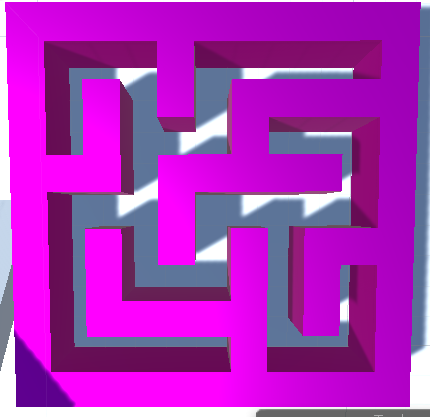
\includegraphics[width=0.5\textwidth]{Blocs.PNG}
    \caption{Blocs}
    \label{Blocs}
\end{figure}{}

\par\vspace{0.5cm}
\begin{figure}[!h]
    \centering
    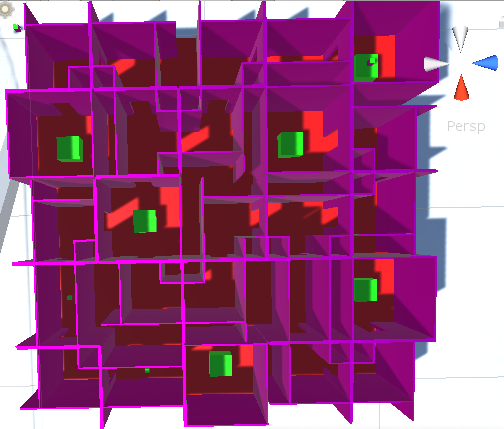
\includegraphics[width=0.5\textwidth]{Salles.PNG}
    \caption{Salles}
    \label{Salles}
\end{figure}{}

\newpage
\subsection{A faire}

Voici les tâches à travailler avant la prochaine soutenance :

\begin{itemize}
\item Gameplay du joueur : Le joueur peut se déplacer correctement mais la plupart des événements ne sont pas synchronisés entre joueurs comme le status.
\item Gameplay du jeu : Ici aussi, il faudra synchroniser les événements de jeu comme les phases, la partie la plus importante du jeu (sans elle il n'y a aucun gameplay).
\item Effets : Cette partie ne me semble pas prioritaire pour le moment mais une fois que les autres tâches auront été avancé, donner un peu plus de vie au jeu en rajoutant quelques effets pourrait s'avérer utile.
\end{itemize}


\subsection{Conclusion}

Pour conclure, je pensais pouvoir avancer un peu plus vite pour implémenter les phases du jeu mais il a été difficile de prévoir tous les événements réseau et nous avons préféré éviter les bugs lors de cette soutenance et présenter un jeu propre et sans vrai gameplay.
Pour la prochaîne soutenance, le premier but sera d'avoir un gameplay en évitant les mauvaises synchronisations en réseau.



%%%%%%%%%%%%%%%%%%%%%% Steve %%%%%%%%%%%%%%%%%%%%%%
%%%%%%%%%%%%%%%%%%%%%% Conclu %%%%%%%%%%%%%%%%%%%%%%
%%%%%%%%%%%%%%%%%%%%%% Annexes %%%%%%%%%%%%%%%%%%%%%
 
\newpage
\section{Annexes}


%%%%%% Celian %%%%%
\subsection{Célian}
\subsubsection{Mouvements}
\label{Mouvements}
\begin{lstlisting}
// If input and (not max speed or braking)
if (movements.sqrMagnitude > .1 &&
    (tangentSpeed < maxSpeed * maxSpeed * speedFactor * speedFactor ||
    velocity.x * movements.x + velocity.z * movements.z < 0))
        velocity += movements * Time.deltaTime * speedFactor;
\end{lstlisting}

\subsubsection{Friction}
\label{Friction}
\begin{lstlisting}
// Friction
if (grounded)
{
    velocity.x -= velocity.x * Time.deltaTime * friction;
    velocity.z -= velocity.z * Time.deltaTime * friction;
}
else
{
    velocity.x -= velocity.x * Time.deltaTime * damping;
    velocity.z -= velocity.z * Time.deltaTime * damping;
}
\end{lstlisting}


\subsubsection{Réseau (A)}
\label{NetA}
\begin{lstlisting}
// Ce code est raccourci

// The player controlled by the client
public static Player localPlayer;

// List of all players (as GameObject)
public static List<GameObject> Players;

// Registers a new player in the players list
public static void RegisterPlayer(GameObject p)
{
    // Update the player list
    players.Add(p);

    if (players.Count == PhotonNetwork.PlayerList.Length)
        // Dispatch events
        OnAllPlayersInGame();
}
\end{lstlisting}


\subsubsection{Réseau (B)}
\label{NetB}
\begin{lstlisting}
// When the player controlled by the client hits another player
void OnControllerColliderHit(ControllerColliderHit hit)
{
    // The player collides another player
    // This player must send the event
    if (net.HasPriority(pNet))
    {
        // This player is infected
        if (state.Status == PlayerState.PlayerStatus.HEALED &&
            pState.Status == PlayerState.PlayerStatus.INFECTED)
            PlayerNetwork.SendPlayerStatusSet(net.id, PlayerState.PlayerStatus.INFECTED);
        // The other player is infected
        else if (pState.Status == PlayerState.PlayerStatus.HEALED &&
            state.Status == PlayerState.PlayerStatus.INFECTED)
            PlayerNetwork.SendPlayerStatusSet(pNet.id, PlayerState.PlayerStatus.INFECTED);
    }
}
\end{lstlisting}


\subsubsection{Phases}
\label{PhaseA}
\begin{lstlisting}
public enum PlayerStatus
{
    INFECTED,
    HEALED,
    CORRUPTED,
    GHOST
}

public PlayerStatus Status
{
    set
    {
        // Update status
        status = value;

        // Change label
        if (player && player.nameUi)
            player.nameUi.SetStatus(status);

        // Update material / play sound...
        switch (status)
        {
            case PlayerStatus.HEALED:
                Debug.Log("Player has status HEALED");
                break;
            case PlayerStatus.INFECTED:
                Debug.Log("Player has status INFECTED");
                break;
        }
    }
}
\end{lstlisting}

\subsubsection{Animations}
\label{Animations}

\begin{figure}[h]
	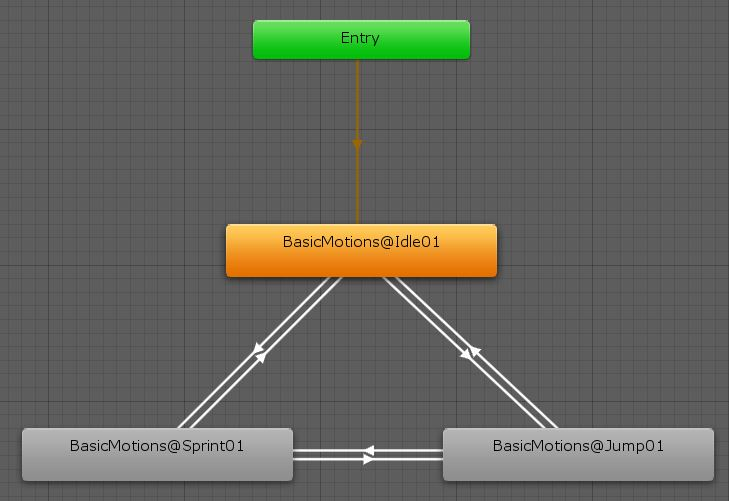
\includegraphics[width=1\textwidth]{anim.jpg}
	\caption{Schéma d'animations}
\end{figure}



\newpage
\end{document}










%%% TODO :
% Certaines partie de code sont non colorisees


